\section{Balls Localization and Segmentation}

To solve the ball localization and segmentation sub-tasks the following algorithm was implemented.
The latter goes through the following three major steps:
\begin{enumerate}
    \item Region proposals generation
    \item False positive filtering
    \item Bounding boxes refinement
\end{enumerate}
\noindent
Before starting with the actual algorithm presentation, a few consideration must be made.
Exclusively for this project part, the used first video frame is the one contained in the given "frames" folder, which is different
from the one taken directly from the video using OpenCV due to compression factors. This choice was made because better system performance relative to 
ball localization and segmentation were obtained using the former.

Furthermore, this section only accurately covers the Ball Localization task solution, showing how the final set of bounding boxes is obtained.
The adopted solution for the Balls Segmentation task, simply consists in creating a mask obtained by fitting a circle inside the found bounding boxes.
As it will explained, the boxes were constrained to be squared, so this operation was trivial.


\subsection{Region proposals generation}
This first step of the algorithm aims to generate regions of interest that will very likely 
contain a ball. The idea behind this step is to find circular regions in the image and create for each one of them
a bounding box to contain it. To do this, the Hough Transform algorithm applied to circles was adopted
(\textit{HoughCircles()} in OpenCV).

Although, the algorithm wasn't applied directly on the grayscale version of the image since
this would have lead to a great number of false positives and false negatives. 
The false positive origin from circles in the image coming from objects in the table different from the balls.
False negatives instead are caused by some balls having almost exactly the same grayscale pixel intensity value of the table cloth,
making \verb|HoughCircles| unable to detect them.
For this algorithm step, the aim is to nullify the number of false negatives, ensuring that every ball is covered by bounding box.
The removal of false positives from the set of found boxes is covered by the second step of the algorithm.

A pre-processing that highlights the balls in the table was needed in order to ease the detection via \verb|HoughCircles|.
The first try involved \verb|K-means| clustering in the color space. Ideally, with parameter \verb|K| big enough, table and balls should have been
clustered in different sets given the differences in color. Although, given the great number of table cloth color variations caused by major illumination
differences between table areas, a great number of found centroids belonged to the table instead of the balls, leading to many balls being clustered
into table regions. Given this result, the second try involved associating each pixel with the closest center (Euclidean distance) in the color space given a pre-defined sets of centers.
The latters were manually defined as ideal ball colors and estimated table cloth color (this estimation is explained later in this section).
In this way it was possibile to correctly clusterize all table pixels but with the inconvenience of including some balls to the table cluster, since the estimated
cloth color was closer to the pixel intensity that the respective ideal ball color. This problem is caused mostly by the fact that the illumination condition of the balls
makes the ball much darker than it actually is. To counteract this issue, additional centers were added to the set exploiting the "value" channel of the HSV enconding
the generate darker variations of the ball colors. Despite the higher quality of the newly found clustering, a few false negatives were still generated.
The cause of this issue was still the extreme color similary between some balls and table cloth. More specifically, if a dark green ball is located in a poorly lit 
region of a green table, the ball became undetectable. Same reasoning for the blue case.

The best image pre-processing found with respect to the aim of this algorithm step, proved to be the following.
Firstly, the mask obtained through the table segmentation was used to isolate the table in the image
in order to constrain HoughCircles to detect circles only inside the table (Figure \ref{fig:masking}). 
\begin{figure}[h!]
    \centering
    \begin{subfigure}[b]{0.45\textwidth}
        \centering
        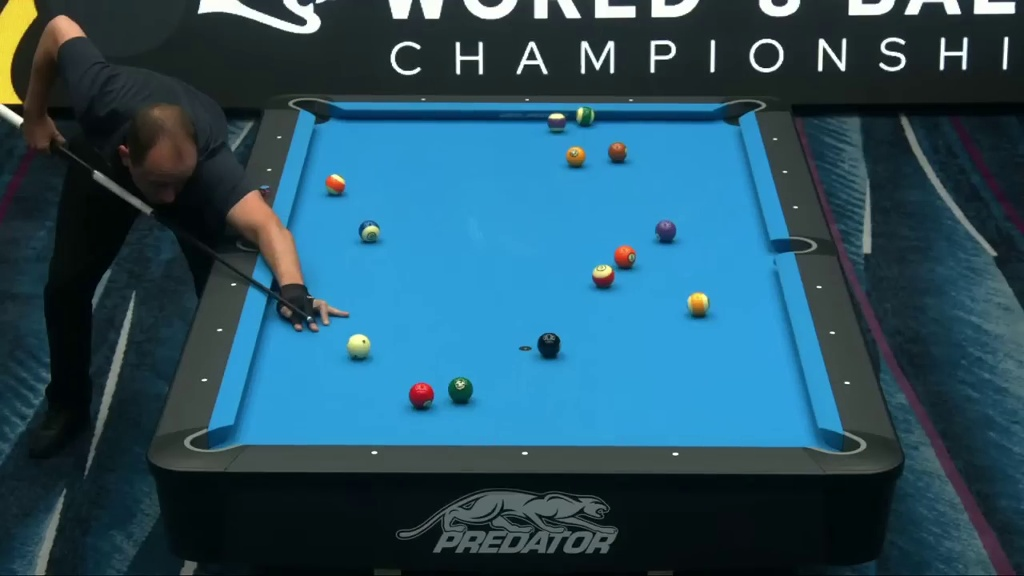
\includegraphics[width=\textwidth]{imgs/ball_localization/original.jpg}
        \caption{Original image}
    \end{subfigure}
    \hspace{0.05\textwidth}
    \begin{subfigure}[b]{0.45\textwidth}
        \centering
        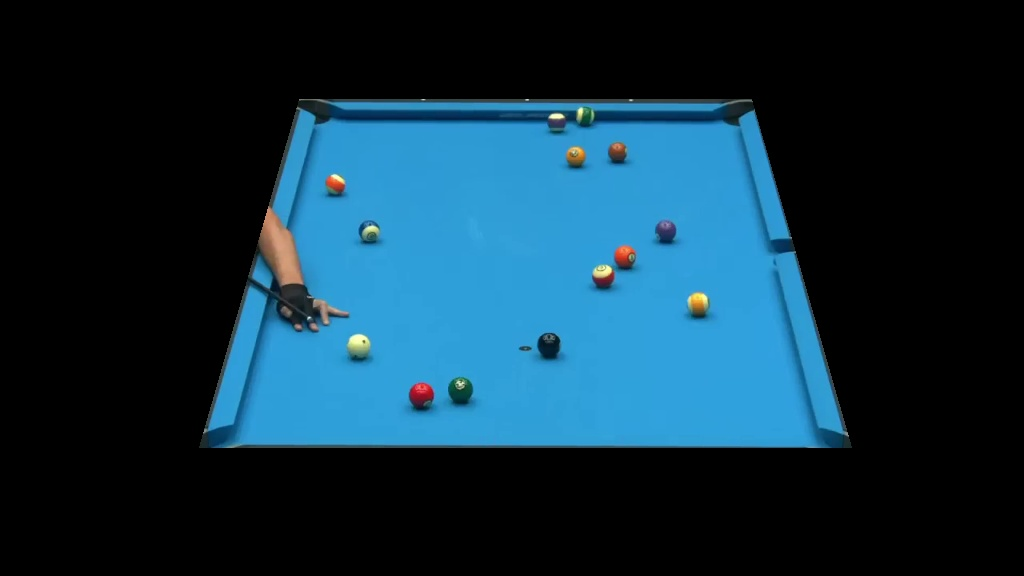
\includegraphics[width=\textwidth]{imgs/ball_localization/masked.jpg}
        \caption{Masked image}
    \end{subfigure}
    \caption{Removal of regions outside of the table one (game1\_clip4)}
    \label{fig:masking}
\end{figure}

Secondly, to ease to detection of circles relative to balls in the table, the following local operation applied to the image pixels
proved to be very effective. Since the table area is mostly empty, the pixel intensity of the table
was evaluated as the mean intensity of non-zero value pixels in the masked image. After this, each non-zero pixel
was set to the absolute value of the difference between the pixel intensity and the evaluated table one.
In this way, all table pixels were set at a value close to zero and instead the balls at a higher intensity
across at least one of the three channels due to differences from the table.
This results in an alternative version of the image in which the table is darker and the transition
between table and balls is much more marked (Figure \ref{fig:subtraction}). 
\begin{figure}[h!]
    \centering
    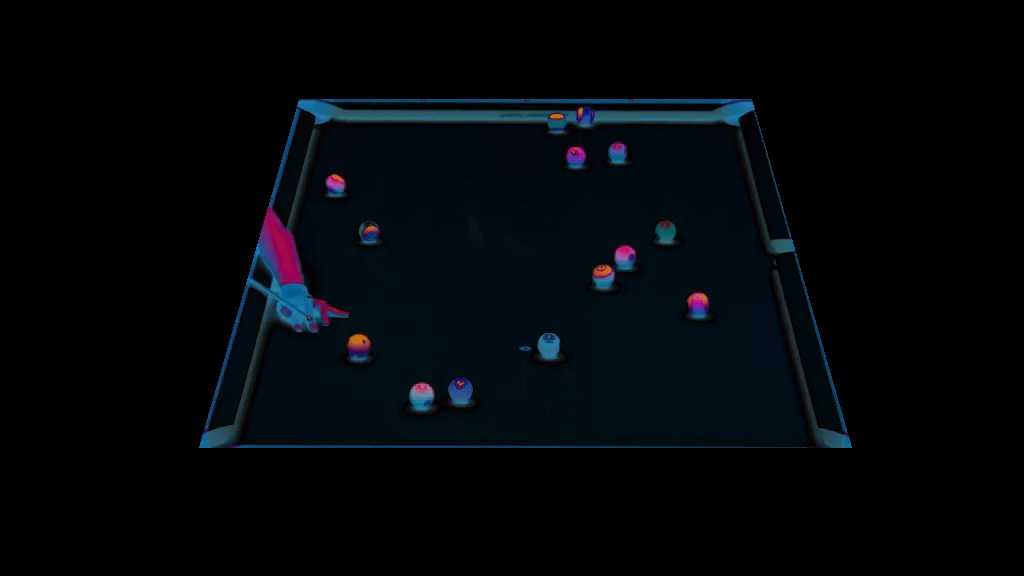
\includegraphics[width=0.85\textwidth]{imgs/ball_localization/subtracted.jpg}
    \caption{Custom local operation is applied to non-zero value pixels (game1\_clip4)}
    \label{fig:subtraction}
\end{figure}

After this, the image was converted to grayscale and HoughCircles was used on it with a general range
of parameters (Method: \verb|Hough_Gradient|, Radius range: 5-15, Distance between circles: \verb|img.rows|/32, Accumulator threshold: 12).
Working only with the BGR version of the image proved to be unsufficient to find all balls because of the 
poor attention to illumination changes of the table color that made impossibile to detect some balls. To solve this issue
the previous steps are performed a second time on the HSV version of the image in order to focus more on 
the colors brightness (value channel). Figure \ref{fig:circles} illustrates an example of these two detections. 
\begin{figure}[h!]
    \centering
    \begin{subfigure}[b]{0.85\textwidth}
        \centering
        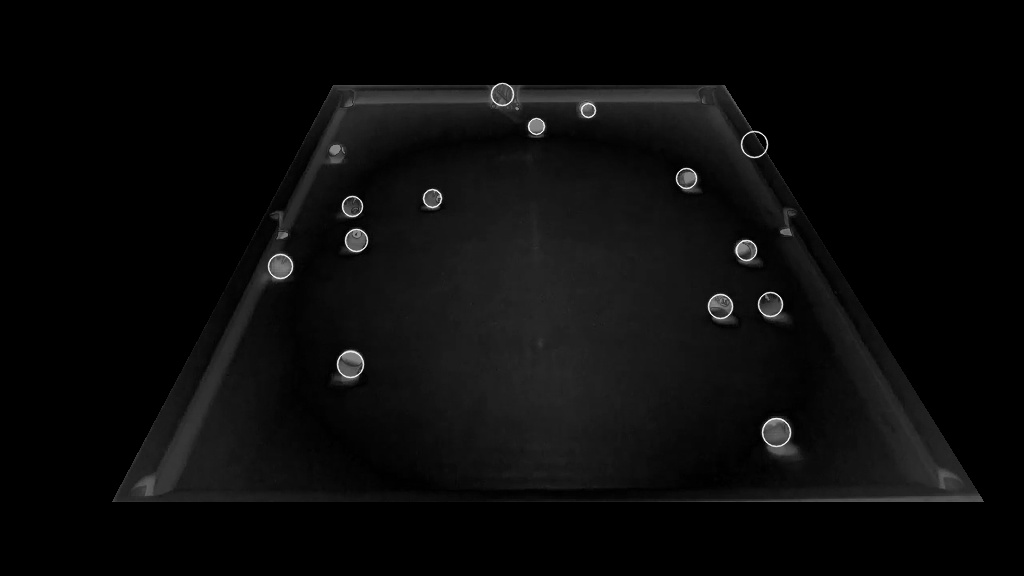
\includegraphics[width=\textwidth]{imgs/ball_localization/circlesBGR.jpg}
        \caption{starting with the BGR version}
    \end{subfigure}
    % \hspace{0.05\textwidth}
    \\
    \begin{subfigure}[b]{0.85\textwidth}
        \centering
        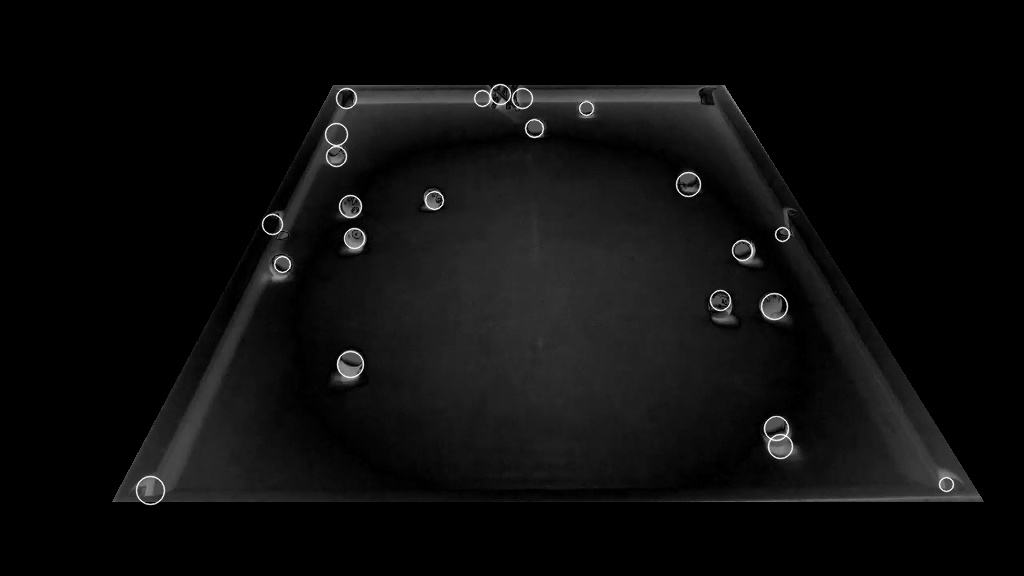
\includegraphics[width=\textwidth]{imgs/ball_localization/circlesHSV.jpg}
        \caption{starting with the HSV version}
    \end{subfigure}
    \caption{Circles detected via HoughCircles on the pre-processed image (game2\_clip1)}
    \label{fig:circles}
\end{figure}

Many balls were detected in both iterations so a smart way to merge the detected circles was necessary.
The final vector of circles is generated by adding all the ones found from the BGR version of the image, that proved 
to represent more accurately the ball contours, and every circles obtained from the HSV version that do not overlap with the ones
in the first set. Then, an additional check to remove possible duplicate (overlapping) circles in the merged set is performed.
Figure \ref{fig:circles_final} shows the output of such merge on the previous example. 
\begin{figure}[h!]
    \centering
    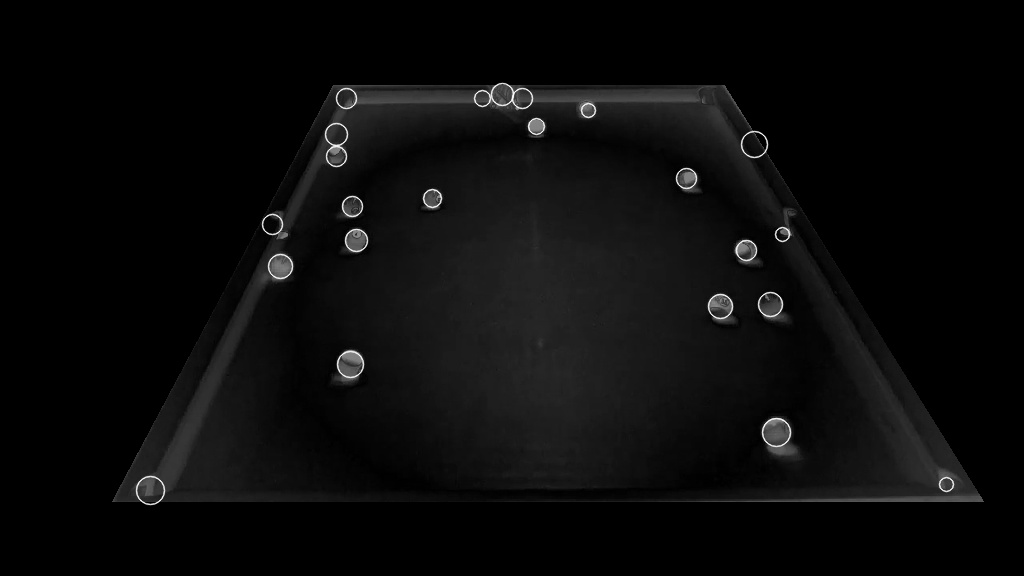
\includegraphics[width=0.85\textwidth]{imgs/ball_localization/circles_merged.jpg}
    \caption{Final set of circles found in the image (game2\_clip1)}
    \label{fig:circles_final}
\end{figure}

Circles were then converted into bounding boxes by creating a Rect object for each circle with abscissa and ordinate equal to the circle ones minus the circle radius,
width and height equal to double the circle radius (diameter).
Through this procedure, for each image a set of bounding boxes is generated, among which exactly one bounding box per ball is contained. 
Figure \ref{fig:fp_detection} shows an example of the results of the procedure upto this point.
\begin{figure}[h!]
    \centering
    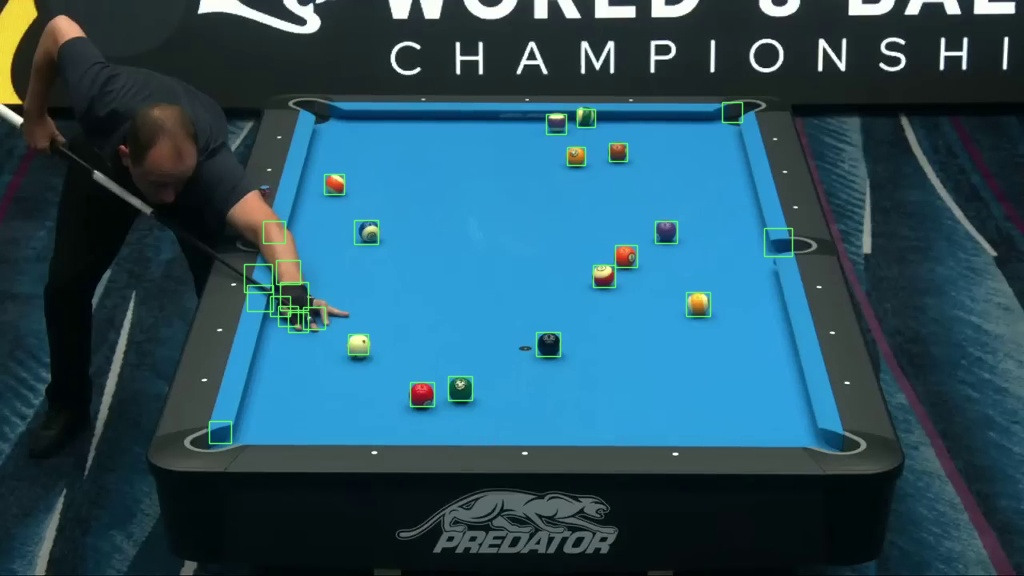
\includegraphics[width=0.85\textwidth]{imgs/ball_localization/fp_detection.jpg}
    \caption{Results of the region proposals generation step (game1\_clip4)}
    \label{fig:fp_detection}
\end{figure}


\subsection{False positive filtering}
As it can be noted from Figure \ref{fig:fp_detection}, to be able to propose regions that cover the whole set of balls in the table, many 
false positive are generated. This happens since there are many circular regions in the table that do not come from any ball.

The first attempt at filtering such false positives resulted in the following algorithm. Given the fact that the balls are always inside the table, the surrounding area
of the detected circles (identified as the circular ring of width double the circle diameter and center equal to the circle one) is supposed to have mean intensity similiar to the table 
cloth one and the mean intensity of the area contained in the circle to be different from it. By estimating the table color
and setting proper distance thresholds in the color space, the implemented filter was able to correctly detect most false positives with a few exceptions.
If the player has his arm particulary stretched on the table, circles detected on his hand were detected as true positives and in case of balls touching the table borders with
width almost imperceptible due to perspective effects, the relative circles were detected as false positives.
These errors were caused by the wrong assumptions initially made.

Because of this, other properties of false and true positives were necessary to be identified in order to create an efficient filter.
The found ones are the following.

False positives can belong to either one of the following two classes: circles relative to holes and circles belonging to the player hand and arm if present 
inside the table region. Additionaly, as it will be later better explained, false positives relative to holes are isolated whereas ones relative to the player are always
grouped together. Using these informations, the following algorithm to filter the false positives was created and implemented.

The filter is composed by two sub-filters placed in cascade to detect the false positives.
The first one operates in the following manner. Given the facts that false positive relative to holes can be found near the longest table
borders, and false positives generated by the player are never isolated (distant from other bounding boxes) since
many circles around the arm and hand are always detected, the filter defines an area inside the projection of the table that excludes
the longest table borders ("safe area") and filters all isolated (non overlapping) bounding boxes which projected center is inside of such area.
To assure that a bounding box is truly isolated, just for this step all boxes width were expanded by a factor $1.5$ so that close but naturally
non-overlapping boxes will now overlap. Figure \ref{fig:safe_area} shows an example of projected table image on which the "safe area" has been drawn.
Note that such rectangle was set at 98\% of the image width and 85\% of its height. These dimensions proved to be effective for the purpose. 
Figure \ref{fig:exp_bboxes} instead shows the result of the bounding boxes expansion applied just for this first filter step. As it can be noticed, close
boxes now overlap, having a better understanding of how much one is isolated.
\begin{figure}[h!]
    \centering
    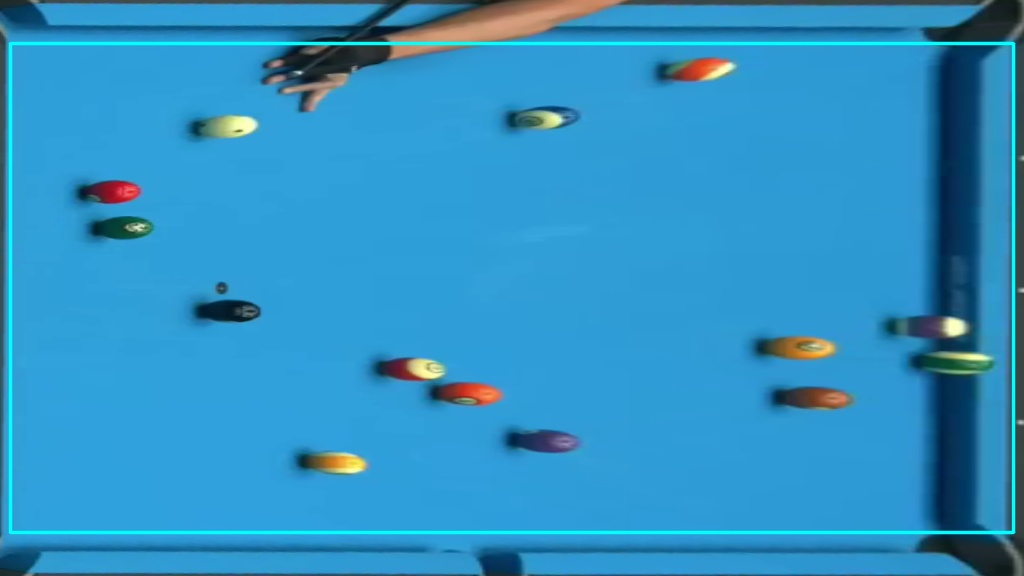
\includegraphics[width=0.85\textwidth]{imgs/ball_localization/safe_area.jpg}
    \caption{Projected table with "safe area" (game1\_clip4)}
    \label{fig:safe_area}
\end{figure}
\begin{figure}[h!]
    \centering
    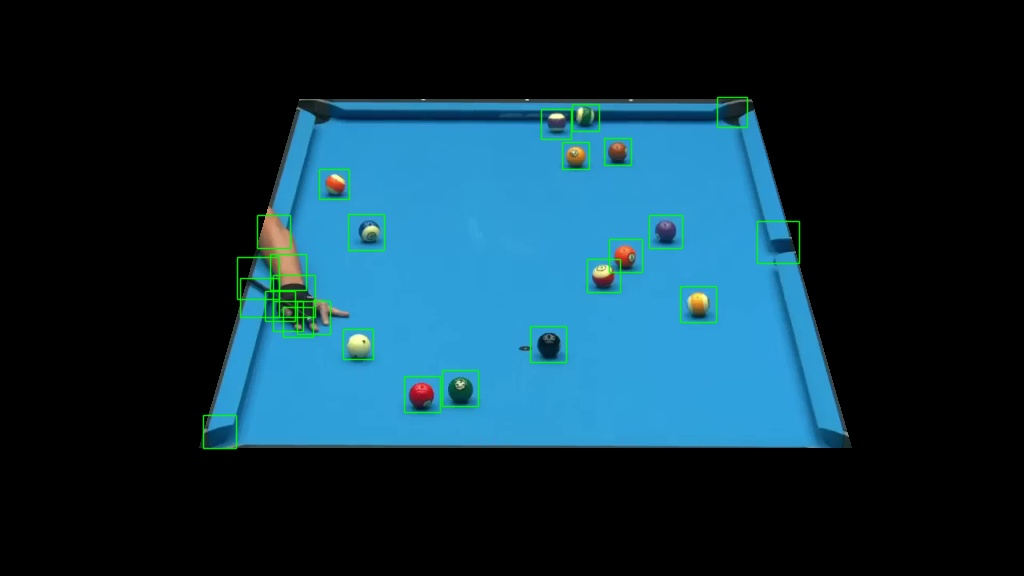
\includegraphics[width=0.85\textwidth]{imgs/ball_localization/exp_boxes_filter.jpg}
    \caption{Expanded bounding boxes in the image (game1\_clip4)}
    \label{fig:exp_bboxes}
\end{figure}

The second and final filter exploits the following property. By dividing the image into connected components, one can notice how found regions belonging to holes, table borders and player arm always
touch the borders of the table projection. This information was exploited to implement the following procedure.
The image is converted in HSV format and the Canny algorithm is applied to the image in order to detect edges.
Then, the projection of the image is obtained using the trasformation matrix returned by the \textit{getTransformation()} function.
This image is then given to the \textit{connectedComponentsWithStats()} method (using Spaghetti labeling algorithm) to obtain
the labeled regions along with useful statistic such the extremal top, bottom, left and right positions of the region.
In this way, a new image is obtained from the transformed canny one by setting at zero all pixels belonging to regions that touch the image
borders or are labeled as background (label 0).
At this point, the percentage of non-zero pixels in each patch of this last image defined by the bounding boxes is computed.
Following our assumptions, all boxes relative to false positives will now contain a low amount of non-zero pixels.
A threshold set at 24\% proved to be effective. Figure \ref{fig:cannyprocess} shows the image resulting from the processing done via \textit{Canny} and \textit{connectedComponentsWithStats}
on which the previously identified bounding boxes are drawn. 
\begin{figure}[h!]
    \centering
    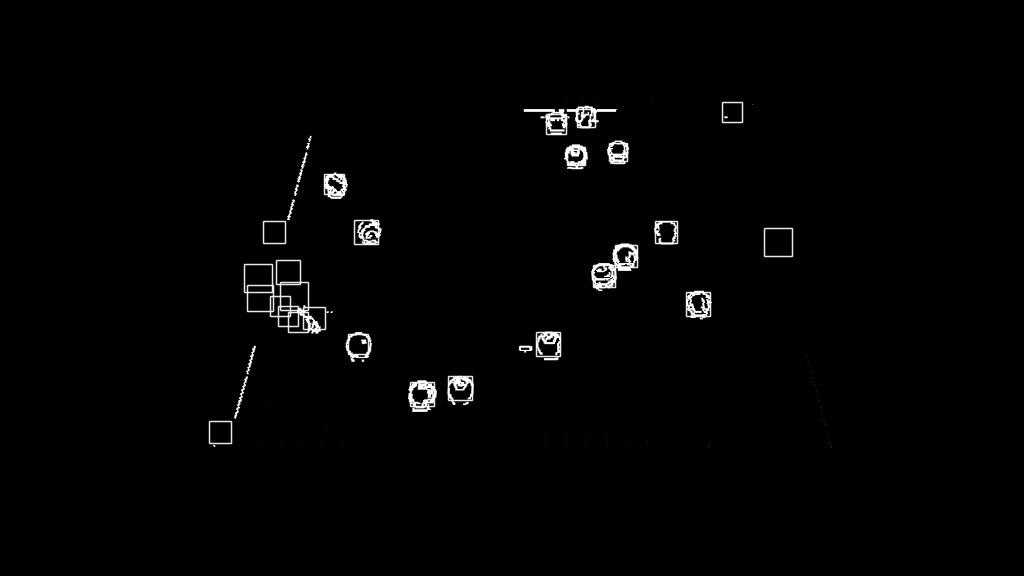
\includegraphics[width=0.85\textwidth]{imgs/ball_localization/conn_comp1.jpg}
    \caption{Results of the canny image processing with bounding boxes (game1\_clip4)}
    \label{fig:cannyprocess}
\end{figure}

Although, this method isn't perfect since it can produce false negatives. In fact, in case of balls close to the borders, their area counted as connected to a component 
of the table border, therefore the respective pixels in the image were set to zero. To fix this kind of errors, a second round of this
procedure is performed but on a new version of the image obtained by running two iterations of the Opening morphological operator with an elliptic 
structuring element of size $(3,2)$. The idea behind this additional step lies in the assumption that table border and balls regions if connected
are weakly connected components. To ensure that no false positive is filtered as true in this last additional step, the percentages
computed during the first iteration are saved into a vector and used during the second in the following manner. If the relative region is no longer touching the image border
and so in the second run the percentage has greatly increased (at least +30\%), then the bounding box is detected as true positive and added
the set of true positives previously computed. Figure \ref{fig:opening} shows an example of this image processing in which when using the Opening operator a ball is disconnected
from the table border and therefore becomes detectable as positive (see the top-left border).
\begin{figure}[h!]
    \centering
    \begin{subfigure}[b]{0.85\textwidth}
        \centering
        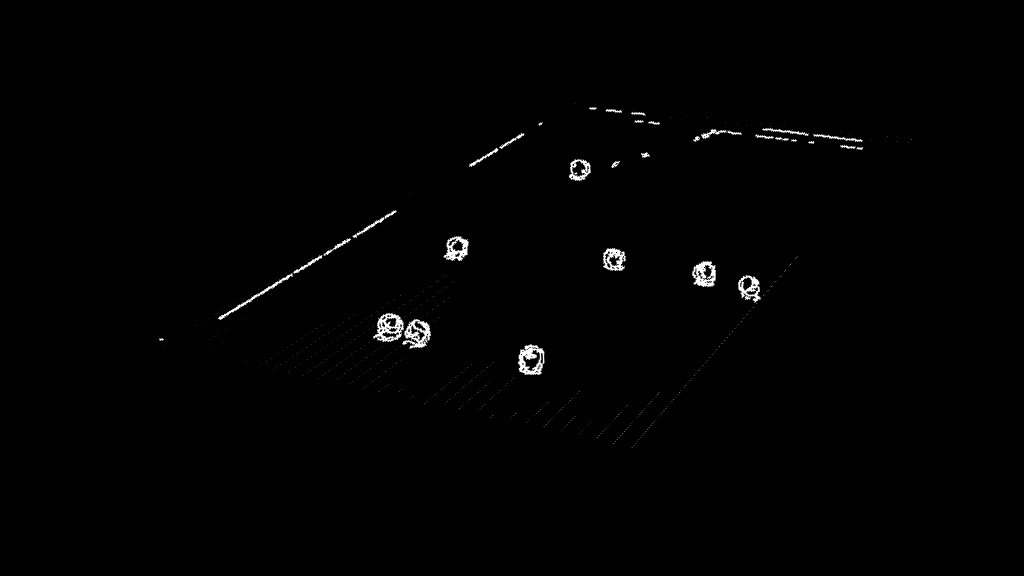
\includegraphics[width=\textwidth]{imgs/ball_localization/final_first.jpg}
        \caption{without Opening (untouched)}
    \end{subfigure}
    % \hspace{0.05\textwidth}
    \\
    \begin{subfigure}[b]{0.85\textwidth}
        \centering
        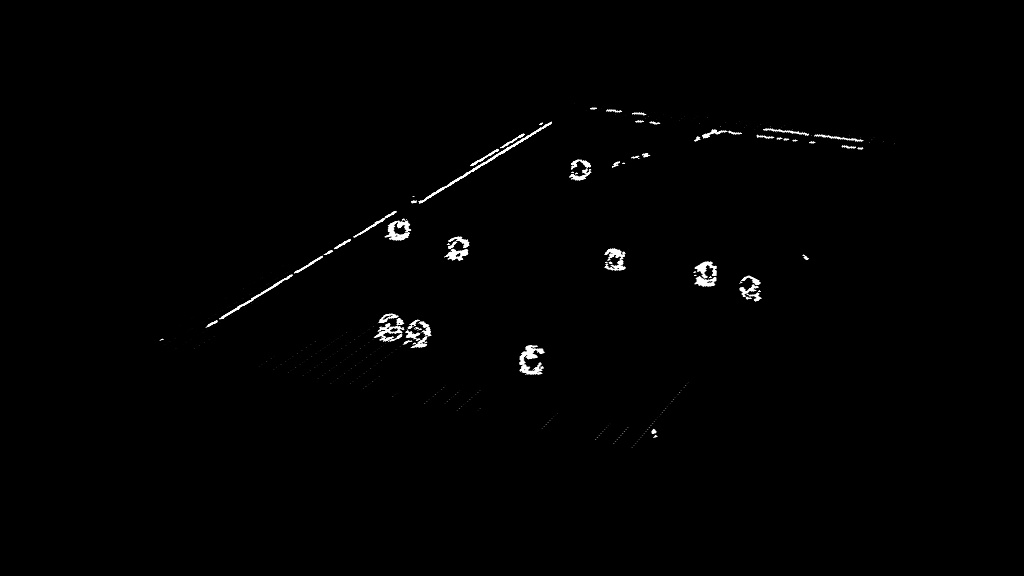
\includegraphics[width=\textwidth]{imgs/ball_localization/final_second.jpg}
        \caption{with Opening (modified)}
    \end{subfigure}
    \caption{Differences in the results of the image processing (game3\_clip1)}
    \label{fig:opening}
\end{figure}

Using this filter, only the regions (bounding boxes) relative to the balls were kept, ensuring a number of false positives and false
negatives equal to zero across the whole provided dataset. Figure \ref{fig:filtering} shows an example of the final results of the complete false positives filtering step of the algorithm.
\begin{figure}[h!]
    \centering
    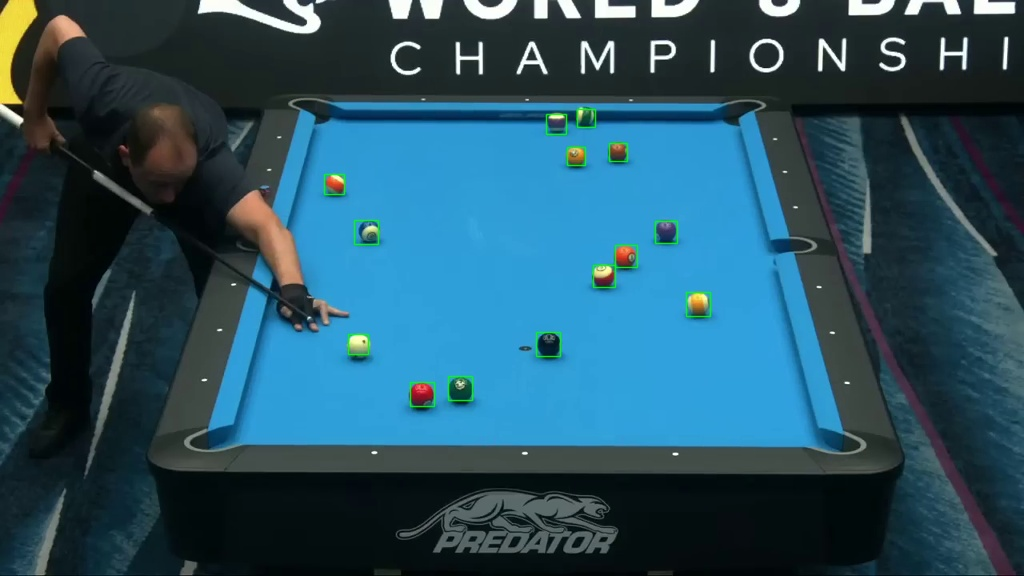
\includegraphics[width=0.85\textwidth]{imgs/ball_localization/filtered_bboxes.jpg}
    \caption{Results of the false positives filtering step (game1\_clip4)}
    \label{fig:filtering}
\end{figure}


\subsection{Bounding boxes refinement}
As suggested by the previous section titles, the found bounding boxes can only be considered as region proposals, since the circles
found through \textit{HoughCircles} in the first step of the detection are not always accurate. This happens because the algorithm was used with a general range of parameters that is supposed to work 
on every possibile image. To obtain the final set of bounding boxes, such regions must be refined.
To do so, we relied once again on \textit{HoughCircles}. To ensure greater precision on the ball circle detection the following operations were carried.
Since in some cases the obtained bounding boxes appeared to be sensibly bigger or smaller than the actual ball shape, to have some reference box dimensions the average
bounding box width was computed. For each box center, a squared mask with dimensions equal to the mean box width multiplied by a scaling coefficient (1.1) is applied to 
the image in such point to focus on the surrounding area around of the ball. The scaling is necessary to ensure that the whole ball appears in the mask image, since the previously computed bounding
boxes are often really tight.

After doing so, \textit{GrabCut} algorithm (\textit{grabCut()} in OpenCV) is used to perform foreground extraction in order to obtain an approximate segmentation of the ball in the masked image in HSV format. 
Then, \textit{HoughCircles} is used on the obtained image with the same set of parameters used before with the exception of the accumulator threshold now set at $10$, and
the radius range that now goes from a third to $70\%$ of the mean bounding box width. The choice on this parameters was made to ensure the detection of circles with true ball dimensions
in the specific image, which were estimated through the mean width computation.

This estimation is valid since at most a few boxes have dimensions sensibly different from the true ones. This information is exploited also to ensure that this refinement
does not worsen the quality of already precise bounding boxes. More precisely, only the bounding boxes for which the detected circle has absolute value of difference between radius and previous box
width halfs greater than $4$ are updated. The update is performed by substituting the previous box with the found circle coverted to bounding box in the manner explained before.
Figure \ref{fig:refine} shows an example in which a ball was not precisely detected in the first step and the respective bounding box is refined by the procedure explained in this section. \\
\begin{figure}[h!]
    \centering
    \begin{subfigure}[b]{0.25\textwidth}
        \centering
        
\includegraphics[width=\textwidth]{imgs/ball_localization/bbox_before.jpg}
        \caption{original box}
    \end{subfigure}
    \hspace{0.05\textwidth}
    \begin{subfigure}[b]{0.25\textwidth}
        \centering
        
\includegraphics[width=\textwidth]{imgs/ball_localization/grabcut.jpg}
        \caption{GrabCut output}
    \end{subfigure}
    \hspace{0.05\textwidth}
    \begin{subfigure}[b]{0.25\textwidth}
        \centering
        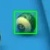
\includegraphics[width=\textwidth]{imgs/ball_localization/bbox_after.jpg}
        \caption{refined box}
    \end{subfigure}
    \caption{Example of bounding box refinement procedure (game1\_clip2)}
    \label{fig:refine}
\end{figure}
It must be noted that sometimes the \textit{GrabCut} algorithm fails to return an accurate ball segmentation since it sometimes considers table borders, holes and shadow of the ball as part of the latter.
In such cases, \textit{HoughCircles} won't find any circles and therefore the relative bounding box won't be updated.
For the same reason, this algorithm is adopted only in this last step and it is not used as backbone of the whole ball localization and segmentation procedure.